\documentclass[a4paper]{article}

% Language setting
% Replace `english' with e.g. `spanish' to change the document language
\usepackage{cite}
\usepackage[utf8]{inputenc}
\usepackage[english]{babel}
\usepackage{xcolor}
% Set page size and margins
% Replace `letterpaper' with `a4paper' for UK/EU standard size
\usepackage[a4paper,top=2cm,bottom=2cm,left=1.5cm,right=1.5cm,marginparwidth=1.75cm]{geometry}

% Useful packages
\usepackage{float}
\usepackage{amsmath}
\usepackage{graphicx}
\usepackage[colorlinks=true, allcolors=blue]{hyperref}
\usepackage{authblk}
\usepackage{tabularx}
\usepackage{longtable}
\usepackage{array}
\usepackage{caption}

% Caption setup
\captionsetup[table]{labelfont=bf, textfont=bf}

\title{\textsf{\textbf{A Brief Review of Gait Recognition Technology}}}
\author[1]{\textbf{Md Abed Afnan}}
\author[2]{\textbf{Saeed Bin Jadid}}
\author[3]{\textbf{Abdullah Al Mamun}}
\author[4]{\textbf{Alauddin mollah}}
\affil[1,2,3,4]{Student, Dept. of CSE, International islamic university chittagong}
\affil[ ]{\{c201004, c211042, c211051, c211055\}@ugrad.iiuc.ac.bd}
\begin{document}
\maketitle

% \begin{abstract}
% Your abstract.
% \end{abstract}
\begin{figure}[!ht]
\centering
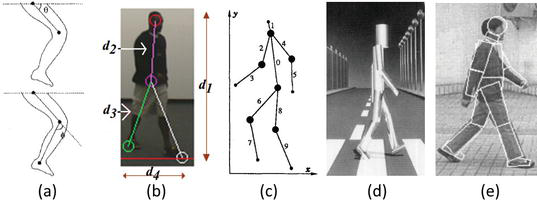
\includegraphics[width=0.7\linewidth]{F2.png}
\end{figure}
\section{\textsf{Introduction}}
Gait recognition is a biometric identification method focusing on individual detection through personal measurements and movement patterns, useful in surveillance and hazy environments where traditional biometric like fingerprints or faces are challenging to use. As technology has advanced over the years, so too has gait recognition technology. Today, there are numerous advanced techniques that can achieve gait recognition more efficiently and robustly.

Gait recognition extends beyond biometric identification and has applications in various fields, including healthcare, sports\cite{2}, gender classification\cite{3}, emotion detection\cite{4}, security etc.

Despite its advantages, gait recognition faces several challenges. One significant challenge is the variability in gait patterns caused by factors such as clothing \cite{9}, carrying conditions \cite{16}, walking speed \cite{7}, and surface type \. These variations can significantly impact the accuracy of gait recognition systems. Additionally, the collection of gait data often requires sophisticated equipment and controlled environments, which may not be feasible in all scenarios. Another challenge is the robustness of the algorithms used. Many advanced techniques, such as deep learning models, require large amounts of data and substantial computational resources. These requirements can limit the applicability of gait recognition in real-time scenarios and resource-constrained environments. Furthermore, the interpretability of these models is often limited, making it difficult to understand how they make decisions and identify potential biases in the recognition process.

This is being seriously considered in gait recognition research. Algorithms Research that generalize well across the environment and conditions. Novel domain adaptation methods tackle this issue they have matured as a field of research recently and substantially enhance the generalization ability of gait recognition systems to different datasets. Efforts are also in place to ensure these models can be deployed even on low resource real-time platforms by making the model weights smaller as well.

This also throws significant research challenges on privacy and ethics. Channels into surveillance, but may begin to cross over the line towards potential abuse and real privacy concerns (eg.ashing onto gaits) An area of research is also that to enable gait recognition systems with a certain grade and deployment use in an ethical practice. This essentially means Make a way to be an Anonymous user.

To conclude, gait is a promising biometric technology and has so many applications as we have discussed. At the same time, it experiences challenges in terms of variability, robustness and ethical considerations. Discussion We have identified several issues plaguing gait recognition algorithms since its inception and ongoing research is working on solving these to correctly improve the accuracy, efficiency, as well utilization of ethics in performing successfully on real-world applications.
\newline\newline
\textbf{Keyword}—Gait Recognition, Biometric Authentication, Deep Learning



\section{\textsf{Literature review}}
\cite{5} In the existing literature on gait recognition, researchers have proposed various approaches that can be broadly categorized into two groups: handcrafted methods and deep learning methods.


Handcrafted methods involve manual extraction of pre-defined features from gait
data. This process typically involves selecting certain characteristics of the gait such as stride length, cadence, and gait rhythm, and using these features to distinguish between individuals. The drawback of handcrafted methods is that they require a significant amount of expert knowledge to identify the appropriate features and may not capture all of the nuances and complexities of gait patterns.


On the other hand, deep learning methods encode intricate features automatically,
without any human intervention. These methods use neural networks to learn the underlying patterns in gait data and identify individuals based on these patterns. Deep learning methods have the advantage of being able to capture more subtle and complex features of gait patterns, leading to improved recognition accuracy compared to handcrafted methods.
\begin{figure}[!ht]
\centering
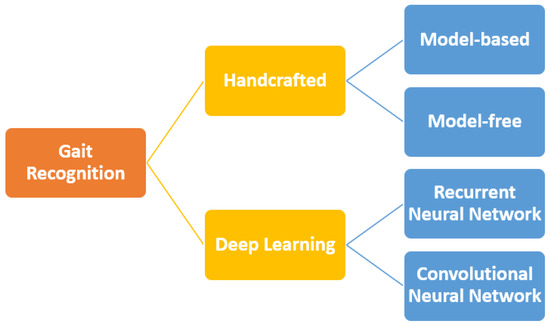
\includegraphics[width=0.53\linewidth]{type-gait.jpg}
\caption{\label{fig:gait}The categorization of gait recognition approach\cite{21}.}
\end{figure}\newline\newline
\textit{\normalsize{\textbf{2.1. Handcrafted Approach}}}\newline
For \cite{6}, a model-based gait recognition technique using Weighted KNN was proposed. The methodology involved transforming Kinect skeletal coordinates into CoB relative coordinates, extracting posture-based features, and classifying them using Weighted KNN. This method required fewer frames for accurate results compared to traditional KNN. Using Dataset-A (self-created) and Dataset-B (Kinect dataset), the performance metrics showed 52\% accuracy for Dataset-A and 88\% to 92\% accuracy for Dataset-B with varying numbers of frames. Limitations included below-average performance in real-world scenarios and the potential for better performance with deep learning approaches.

In \cite{7}, a machine-learning approach for gait recognition was utilized. This involved enhancing motion regions, detecting ROI with optical flow, and using MSVM for recognition. The datasets used were CASIA-A, CASIA-B, and CASIA-C. Performance metrics revealed CCRs of 98.90\%, 95.80\%, and 97.30\% for CASIA-A, CASIA-B, and CASIA-C respectively. However, the method showed reduced accuracy with multiple cameras and was designed primarily for static environments.

A gait analysis system using pressure sensors and an IMU sensor to classify gait phases was developed in \cite{8}. The system employed a PSO-SVM algorithm to enhance classification accuracy. Data was collected from eight healthy adults aged 21-28, using sensors placed on the insole and tongue to measure ground reaction forces (GRF) and foot angle changes. The PSO-SVM classifier achieved 95\% accuracy, outperforming standard SVM and KNN classifiers. However, the study’s small sample size and controlled treadmill environment limit the generalizability of the results.

In \cite{9}, a gait recognition system using Kinect Skeletal Tracking was presented to identify individuals wearing loose-fitting garments. The system recorded gait sequences of 23 participants and stored the coordinates of 25 joints, classifying them using KNN with K=11. Performance metrics included accuracy, sensitivity, specificity, precision, recall, and F-score. The system achieved 92.75\% accuracy for combined joints and 91.30\% accuracy in online testing. Limitations included the challenge of detecting joints obscured by loose-fitting garments and potential environmental factors affecting sensor performance.\newline\newline
\textit{\normalsize{\textbf{2.2. Deep Learning}}}\newline
In \cite{10}, recent advancements in gait recognition using deep learning techniques were reviewed. This included CNNs, LSTM networks, Autoencoders, CapNet, DBN, and GANs, utilizing datasets like CASIA B, OU-ISIR, whuGAIT, and SZU RGB. LSTM models demonstrated robustness on CASIA B and OU-ISIR, while autoencoder models achieved 86\% Rank-1 and 95\% Rank-5 accuracy on the OU-ISR Large Population dataset. However, the main limitations were dataset variability, incomplete movement cycles, and the computational expense of deep learning models.

The work in \cite{11} aimed to improve gait recognition by combining global and local features through the GaitGL framework. This framework uses a Global and Local Convolutional Layer (GLCL) to capture both overall context and fine-grained details. Datasets included CASIA-B, OU-MVLP, GREW, and Gait3D, with performance accuracies of 93.6\% on CASIA-B and 98.7\% on OU-MVLP. Challenges included variable walking conditions, dependence on data quality, and complexity in implementing local feature extraction.

Gait Orientation-based Unsupervised Domain Adaptation (GOUDA) was presented in \cite{12} to address the domain gap in gait recognition due to viewing angle bias. The method used GOUDA with datasets like CASIA-B, OU-MVLP, GREW, and Gait3D. Performance in ablation experiments showed that GOUDA achieved Rank-1 accuracies of 92.8\% across all 11 views when adapting from OU MVLP (source) to CASIA-B (target). The limitations included data variability, dependence on data quality, and implementation complexity.

In \cite{13}, a novel gait recognition approach using the Vision Transformer (ViT), referred to as Gait-ViT, was introduced. This process involves embedding layers, a Transformer encoder, and a multi-layer perceptron for classification. The method, Gait-ViT, processes gait cycles by averaging images, splitting patches, embedding patches, and applying attention mechanisms. The datasets used were CASIA-B, OU-ISIR D, and OU-LP. Results indicated an accuracy of 99.93\% on CASIA-B, 100\% on OU-ISIR D, and 99.51\% on OU-LP. However, data variability, dependence on data quality, and implementation complexity were noted as limitations.

A methodology involving Gait Energy Image (GEI) creation, feature extraction with DenseNet-201, VGG-16, and Vision Transformer (ViT), and ensemble prediction was employed in \cite{14}. The datasets used included CASIA-B, OU-ISIR Dataset D, and OU-ISIR. The Gait-CNN-ViT approach achieved 100\% accuracy on CASIA-B and OU-ISIR, and 99.72\% on OU-LP. The limitations highlighted were generalization to real-world scenarios, data dependency, and implementation complexity.

A novel skeletal gait representation named "skeleton map" and a skeleton-based method called "SkeletonGait" were introduced in \cite{15}. This approach involved generating Gaussian maps for joints and limbs, forming a silhouette-like image. The methods included Skeleton Map Generation, SkeletonGait, and SkeletonGait++, which combines skeleton maps and silhouette features using a fusion-based multi-branch architecture. Datasets used were OU-MVLP, GREW, Gait3D, SUSTech1K, and CCPG. SkeletonGait++ achieved state-of-the-art performance, with a rank-1 accuracy of over 85\% on the challenging GREW dataset. However, potential improvements on the GREW dataset and the absence of frame-by-frame alignment for the OU-MVLP dataset were noted as limitations.

Authors of \cite{16} have leveraged parallel-running custom kernels within a Convolutional Neural Network (CNN) framework to extract features from Gait Energy Image (GEI) images. Their methodology prioritizes dynamic areas like legs and minimizes the influence of static areas affected by covariates. The key method employed is the Custom Kernel CNN. They used datasets CASIA-A and CASIA-C. Performance metrics showed 90\% accuracy for subjects wearing bags and 58\% accuracy for those wearing coats, with an average accuracy of 81.2\%. The study's limitations include the low accuracy for covariates with coats and the potential for improvement through transfer learning.

GFM-Net, a hybrid deep-learning framework using AutoEncoder, CNN, RNN, LSTM, and GRU for gait phase recognition, was developed in \cite{17}. The Gaussian Probability Fusion Module (GFM-Net) optimizes feature fusion using IMU data. Performance metrics revealed 96.7\% accuracy and 86.5\% macro-F1. However, the limitation was macro-F1's complexity in extraction.

In \cite{18}, a deep neural network model for recognizing sensor-based movements from multivariate time series data was proposed. The model used CNNs and hybrid models combining CNNs with LSTM and GRU, employing PCA for dimensionality reduction and class weighting to address class imbalance. Tested on CASIA-B and a custom dataset, the model achieved 94.3\%-94.7\% accuracy on CASIA-B and 98.71\% accuracy on the custom dataset. Challenges included class imbalance, increased computational complexity of hybrid models, and variability in performance on unseen data.

Authors of \cite{19} introduced a gait recognition model capturing spatio-temporal features using the Focal Convolution Layer and Micro-motion Capture Module (MCM). The model processes gait silhouettes frame by frame, using Frame-level Part Feature Extractor (FPFE) and Temporal Feature Aggregator (TFA) with parallel MCMs. The model achieved an average rank-1 accuracy of 87.1\% on the CASIA-B dataset and state-of-the-art performance on the OU-MVLP dataset. Limitations include the need for detailed comparisons with other methods, potential generalizability issues, and unaddressed computational complexity concerns.

A self-supervised learning (SSL) approach with the DINO model to pretrain a feature extractor using a vision transformer (ViT) architecture for automatic gait feature extraction was utilized in \cite{20}. A fully connected neural network classifier was then trained using a supervised learning approach. The methodology was validated on CASIA-B and OU-MVLP datasets, achieving an accuracy of 99.64\% on CASIA-B with the ViTs16 model. Despite its high performance, real-world challenges like illumination changes, occlusions, and varying environmental conditions were not fully addressed. Additionally, computational costs and the robustness of learned features required further investigation. This approach falls under the category of deep learning due to the use of SSL and vision transformers.





\begin{center}
\begin{longtable}{|>{\raggedright\arraybackslash}p{0.5cm}|>{\raggedright\arraybackslash}p{1.3cm}|>{\raggedright\arraybackslash}p{0.9cm}|>{\raggedright\arraybackslash}p{2.3cm}|>{\raggedright\arraybackslash}p{2.8cm}|>{\raggedright\arraybackslash}p{2cm}|>{\raggedright\arraybackslash}p{2.3cm}|>{\raggedright\arraybackslash}p{2.5cm}|}
\caption{Reviewed articles summarization} \\
\hline
\textbf{Ref} & \textbf{Journal} & \textbf{Year} & \textbf{Methodology} & \textbf{Methods} & \textbf{Dataset} & \textbf{Performance} & \textbf{Limitation} \\
\hline
\endfirsthead
\hline
\textbf{Ref} & \textbf{Journal} & \textbf{Year} & \textbf{Methodology} & \textbf{Methods} & \textbf{Dataset} & \textbf{Performance} & \textbf{Limitation} \\
\hline
\endhead
\hline
\endfoot
\endlastfoot

\cite{6} & IOE & 2020 & Proposed a model-based gait recognition technique using Weighted KNN. & Weighted KNN(WKNN) & Dataset-A(self-created), Dataset-B(Kinect datase) & 52\% accurate on Dataset-A, Dataset-B got 88\% to 92\% of different frame. & In realworld scenario it can perform bellow average. also Dataset-A got only 52\% accuracy. \\
\hline

\cite{7} & IGI Global & 2020 & This paper used Multi-class support vector machine (MSVM) utilization for recognition. & Multi-class support vector machine (MSVM) & CASIA-A, CASIA-B, CASIA-C & On CASIA-A: 98.90\%, CASIA-B: 95.80\%, and CASIA-C: 97.30\% & Dynamic environment is not compatible with this approach because it is proposed for static environment.\\
\hline

\cite{8} & Eng. Letters & 2024 & Gait analysis using pressure sensors and IMU, classified with PSO-SVM. & PSO-SVM & Eight healthy adults & 95\% accuracy. & Small sample size, controlled environment. \\
\hline

\cite{9} & IAJIT & 2024 & Gait recognition using Kinect Skeletal Tracking. & Kinect Skeletal Tracking, KNN & 23 individuals, 35 samples each & Combined top three joints: 92.75\% accuracy, online testing: 91.3\%. & Clothing impact, environmental factors, sample size. \\
\hline

\cite{10} & ACM & 2022 & Review of gait recognition using deep learning. & CNNs, LSTM, Autoencoders, CapNet, DBN, GANs. & CASIA B, OU-ISIR, whuGAIT, SZU RGB & Autoencoder 86\% Rank-1, 95\% Rank-5 on OU-ISR; Models >91\% combining accelerometer and gyroscope data. & Dataset variability, incomplete data, model complexity. \\
\hline

\cite{11} & AAAI & 2023 & Improve accuracy by utilizes a new type of convolutional layer, the Global and Local Convolutional Layer (GLCL) & GLCL, LTA & CASIA-B, OU-MVLP, GREW, Gait3D & CASIA-B 93.6\%, OU-MVLP 98.7\%, GREW 68.0\%, Gait3D 63.8\%. & Variable walking conditions, data dependence, implementation complexity. \\
\hline

\cite{12} & CVF & 2024 & Gait Orientation-based method for Unsupervised Domain Adaptation (GOUDA). & GOUDA & CASIA-B, OU-MVLP, GREW, Gait3D & 92.8\% Rank-1 accuracy on OU MVLP to CASIA-B. & Data variability, dependence on data quality, implementation complexity. \\
\hline

\cite{13} & Sensors & 2022 & Gait recognition using Vision Transformer (Gait-ViT). & Gait-ViT: Embedding layers, Transformer encoder, MLP. & CASIA-B, OU-ISIR D, OU-LP & CASIA-B 99.93\%, OU-ISIR D 100\%, OU-LP 99.51\%. & Data variability, dependence on data quality, implementation complexity. \\
\hline

\cite{14} & Sensors & 2023 & Gait Energy Image (GEI) with CNN and Vision Transformer (ViT). & DenseNet-201, VGG-16, ViT, Gait-CNN-ViT. & CASIA-B, OU-ISIR D, OU-ISIR & 100\% on CASIA-B, OU-ISIR; 99.72\% on OU-LP. & Generalization to real-world, data dependency, implementation complexity. \\
\hline

\cite{15} & Arxiv & 2022 & Introduced a novel skeleton-based method called "SkeletonGait" &  SkeletonGait++ &  OU-MVLP, GREW, Gait3D, SUSTech1K, CCPG & rank-1 with 85\% accuracy on the challenging GREW dataset. & Couldn't get result for OU-MVLP in skeletonGait++.\\
\hline

\cite{16} & Heliyon & 2024 & Proposed a custom kernal CNN to extract features from GEI images.& Custom Kernel CNN & CASIA-A, CASIA-C & wearing bags: 90\% accuracy. wearing coats: 58\% accuracy. Avg. accuracy 81.2\%. & Loss can be lowered by transfer learning \\
\hline

\cite{17} & Wiley & 2020 & This Paper focuses on a hybrid deep-learning framework called GFM-Net & Gaussian Probability Fusion Module(GFM-net) &1. IMU data &  GFM-Net has over 96.7\% accuracy and macro-F1 is up to 86.5\%, & The macro-F1 metric shows some limitations in complexity extraction. \\
\hline

\cite{18} & VJS & 2023 & Gait recognition using deep neural networks on multivariate time series data. & CNN, CNN-LSTM, CNN-GRU, PCA, class weighting & CASIA-B, Custom Dataset & CASIA-B: 94.3\% to 94.7\%, Custom Dataset: Random Forest 98.71\%, SVM 93.58\%, LSTM 94.93\%. & Class imbalance, model complexity, generalization. \\
\hline

\cite{19} & CVF & 2020 & Gait recognition using spatio-temporal features and focal convolution layer. & FPFE, TFA, GaitPart, MCM & CASIA-B, OU-MVLP & CASIA-B: 87.1\%, OU-MVLP: state-of-the-art. & Limited comparison with other methods, generalizability, computational complexity. \\
\hline

\cite{20} & Sensors & 2022 & Gait recognition using self-supervised learning(SSL) with DINO model and ViT. & SSL, DINO, ViT, FCNN & CASIA-B, OU-MVLP & CASIA-B: FCNN 99.64\%, ViTs16 99.64\%. & Real-world challenges, generalizability, computational costs. \\
\hline


\end{longtable}
\end{center}
For detailed information, please refer to the Excel data file. \href{https://docs.google.com/spreadsheets/d/1v_MnKu-NIqDchRvh2tJIpmYFTmqJW6BGVCC40wq-em4/edit?usp=sharing}{Gait recognition}

\bibliographystyle{plain}
\bibliography{sample}

\end{document}